\chapter{Teste de PCI: práticas comuns, desafios atuais e técnicas avançadas}
%\addcontentsline{toc}{chapter}{Teste de PCI: práticas comuns, desafios atuais e técnicas avançadas}

O teste de fim de linha de manufatura realizado nas PCIM é um dos procedimentos de teste finais antes de embalar e entregar o produto. Tipicamente, cada montagem de placa produzida tem que passar em variadas fases de teste antes de ser qualificada para expedição. O montante destas fases de teste pode ser numerosas para um produto eletrônico complexo e depende também da qualidade, e confiabilidade dos seus requerimentos de projeto (Jutman et al., 2014). 

Cada classe de teste é especializada para uma gama limitada de defeitos, e é custoso, senão impossível, forçar a cobertura de defeitos fora daqueles que tal classe tenta resolver. Dessa maneira, a solução normalmente adotada é combinar diversas técnicas de teste (Jutman et al., 2014). Dessa maneira, uma estratégia de teste eficiente para um produto complexo tipicamente requer ao menos uma técnica para cada categoria exibida na Tabela \ref{tab:testcategories}. Considera-se também que combinação de técnicas de teste é também ditada por sua viabilidade econômica \citep{davis1994economics}.

\newpage

\begin{table}[]
\centering
\caption{Principais categorias em teste de Placas de Circuito Impresso montadas - PCIMs. Traduzido de Jutman (2014)}
\label{tab:testcategories}
\begin{tabular}{ll}
\hline
\rowcolor[HTML]{EFEFEF} 
\multicolumn{1}{|l}{\cellcolor[HTML]{EFEFEF}{\color[HTML]{000000} }}                                   & \multicolumn{1}{l|}{\cellcolor[HTML]{EFEFEF}{\color[HTML]{000000} \textit{Pré-reflow: SPI\footnotemark, AOI\footnotemark  }}}                 \\ \cline{2-2} 
\rowcolor[HTML]{EFEFEF} 
\multicolumn{1}{|l}{\multirow{}{}{\cellcolor[HTML]{EFEFEF}{\color[HTML]{000000} \textbf{Inspeção}}}}         & \multicolumn{1}{l|}{\cellcolor[HTML]{EFEFEF}{\color[HTML]{000000} \textit{Pós-reflow: Inspeção Visual, AXI\footnotemark, AOI}}}                 \\
\rowcolor[HTML]{C0C0C0} 
\multicolumn{1}{|l}{\cellcolor[HTML]{C0C0C0}{\color[HTML]{000000} \textbf{Teste Elétrico}}}                     &  \multicolumn{1}{l|}{\cellcolor[HTML]{C0C0C0}{\color[HTML]{000000} \textit{ICT, MDA, FPT\footnotemark}}}           \\
\rowcolor[HTML]{9B9B9B} 
\multicolumn{1}{|l}{\cellcolor[HTML]{9B9B9B}{\color[HTML]{000000} \textbf{Teste de Sondagem}}}                  & \multicolumn{1}{l|}{\cellcolor[HTML]{9B9B9B}{\color[HTML]{000000} \textit{Boundary Scan}}}             \\
\rowcolor[HTML]{656565} 
\multicolumn{1}{|l}{\cellcolor[HTML]{656565}{\color[HTML]{FFFFFF} Teste em alta velocidade}} & \multicolumn{1}{l|}{\cellcolor[HTML]{656565}{\color[HTML]{FFFFFF} Teste centralizado por..}}            \\
\rowcolor[HTML]{343434} 
\multicolumn{1}{|l}{\cellcolor[HTML]{343434}{\color[HTML]{FFFFFF} Instrumentação Embarcada}}           & \multicolumn{1}{l|}{\cellcolor[HTML]{343434}{\color[HTML]{FFFFFF} Instrumentação BIST (Hardware Fixo)}} \\ \hline
\rowcolor[HTML]{000000} 
{\color[HTML]{FFFFFF} Teste Funcional}                                                                 & {\color[HTML]{FFFFFF} Testes de interfaces e etc.}                                                                                 \\ \hline
\end{tabular}
\end{table}
%bug
\footnotetext[1]{Inspeção de pasta de solda ou em inglês: \textit{Solder Paste Inspection -- SPI}}
\footnotetext[2]{Inspeção Ótica Automatizada ou em inglês \textit{Automated Optical Inspection -- AOI}}
\footnotetext[3]{Inspeção Radiográfica Automatizada ou em inglês \textit{Automated X-Ray Inspection -- AXI}}
\footnotetext[4]{Respectivamente: Teste In-Circuit, Manufacturing Defect
Analysis, Flying Probe Test}

\section{Sondagem periférica para a inspeção de PCIM}

Técnicas de inspeção ajudam a checar a integridade geral da placa montada como presença de componentes, polaridade, qualidade de solda, pinos levantados, etc. E conforme Jutman (2014), testes de sondagem periférica - como o JTAG / \textit{Boundary Scan} -  são hoje o padrão da industria de teste em nível de placa pois promovem uma tecnologia de teste barata e eficiente em termos de cobertura e capacidade de resolução de problemas \nocite{parker2012boundary}. O iNEMI fez uma pesquisa em 2009 \citep{geiger2009boundary} que corroboa isso: aproximadamente 80\% dos engenheiros de teste consideram de importância alta ou moderada a inserção de testes de sondagem periférica como uma de suas táticas de verificação de seus produtos, até mesmo pela redução no custo de geral desenvolvimento que essa categoria de teste promove (Jutman et al., 2014). 

Na tabela \ref{tab:boundaryscanfamily}., podemos ver a todas as variações de Sondagem periférica e suas respectivas finalidades. O padrão IEEE 1149.1 \citep{ieee11491old} é o antecessor de toda a família e prove o conceito básico da arquitetura e os princípios de acesso de teste (Jutman et al., 2014). A última versão do IEEE 1149.1 foi publicada em 2013 \citep{ieee11491yr2013} com grandes atualizações incorporadas, incluindo padronizações de meios de controle de instrumentação embarcada e condicionamento de sinais a nível de pinagem.

\begin{table}[]
\centering
\tiny
\caption{Padrões IEEE de acesso ao teste baseado em sondagem. Adaptado de Jutman (2014)}
\label{tab:boundaryscanfamily}
\begin{tabular}{p{50}p{50}p{50}p{50}}
\hline
\rowcolor[HTML]{C0C0C0} 
\multicolumn{1}{|p{50pt}|}{\cellcolor[HTML]{C0C0C0}\textbf{Foco principal de aplicação}} & \multicolumn{1}{p{50pt}|}{\cellcolor[HTML]{C0C0C0}\textbf{Propósito Principal}} & \multicolumn{1}{p{50pt}|}{\cellcolor[HTML]{C0C0C0}\textbf{Base da Tecnologia}}    & \multicolumn{1}{p{50pt}|}{\cellcolor[HTML]{C0C0C0}\textbf{Classes de falta a serem cobertas}}     \\
\rowcolor[HTML]{656565} 
\multicolumn{4}{|l|}{\cellcolor[HTML]{656565}{\color[HTML]{FFFFFF} \textbf{IEEE 1149.1 - Boundary Scan \citep{ieee11491old, ieee11491yr2013}}}}                                                                                        \\
\multicolumn{1}{|p{50pt}|}{Teste de Manufatura de PCI}                                        & \multicolumn{1}{p{50pt}|}{Melhorias de acesso aos testes}                               & \multicolumn{1}{p{50pt}|}{Registradores de sondagem on-chip}                            & \multicolumn{1}{p{50pt}|}{Faltas em pinos e integridade de circuto}                                 \\
\rowcolor[HTML]{656565} 
\multicolumn{4}{|l|}{\cellcolor[HTML]{656565}{\color[HTML]{FFFFFF} \textbf{IEEE 1149.4 - Barramento para testes de sinais mistos \citep{ieee11494} .}}}\\

\multicolumn{1}{|p{50pt}|}{Medição de sinais analógicos} &
\multicolumn{1}{p{50pt}|}{Melhorias de acesso aos testes} & 
\multicolumn{1}{p{50pt}|}{Chaves \textit{on-chip}} &
\multicolumn{1}{p{50pt}|}{Valores paramétricos}\\

\rowcolor[HTML]{656565} 
\multicolumn{4}{|l|}{\cellcolor[HTML]{656565}{\color[HTML]{EFEFEF} \textbf{IEEE 1149.6 - Teste BST de Redes Digitais Avançadas \citep{ieee11496}}}}\\

\multicolumn{1}{|p{50pt}|}{Teste de redes LVDS de alta velocidade} &
\multicolumn{1}{p{50pt}|}{Teste de malhas acopladas em corrente alternada} & 
\multicolumn{1}{p{50pt}|}{Geradores de pulsos \textit{on-chip}} &
\multicolumn{1}{p{50pt}|}{integridade de malha}\\

%\rowcolor[HTML]{656565} 
\multicolumn{4}{|l|}{\cellcolor[HTML]{656565}{\color[HTML]{EFEFEF} \textbf{IEEE 1149.7 - Pinos reduzidos e TAP aprimorado \citep{ieee11497}}}}\\

\multicolumn{1}{|p{50pt}|}{Teste de placa e debug de software} &
\multicolumn{1}{p{50pt}|}{Acesso à teste flexivel e em alta velocidade por dois pinos} & 
\multicolumn{1}{p{50pt}|}{SERDES, endereçamento} &
\multicolumn{1}{p{50pt}|}{Contempla todos acima}\\

%\rowcolor[HTML]{656565} 
\multicolumn{4}{|l|}{\cellcolor[HTML]{656565}{\color[HTML]{EFEFEF} \textbf{IEEE 1149.8.1 - Alternância de pinos e sensoriamento sem contato\citep{ieee114981}}}}\\

\multicolumn{1}{|p{50pt}|}{Teste de interconexão de PCIM} &
\multicolumn{1}{p{50pt}|}{Ligações para componentes passivos} & 
\multicolumn{1}{p{50pt}|}{chapas de sensoriamento capacitivo} &
\multicolumn{1}{p{50pt}|}{Circuitos abertos: AC e DC }\\

\multicolumn{4}{|l|}{\cellcolor[HTML]{656565}{\color[HTML]{EFEFEF} \textbf{IEEE P1149.10- TAP de alta velocidade \citep{ieeep1149102016} }}}\\

\multicolumn{1}{|p{50pt}|}{O mesmo que todos acima} &
\multicolumn{1}{p{50pt}|}{Permutação de dados de teste em alta velocidade} & 
\multicolumn{1}{p{50pt}|}{Reuso de pinos I/O de alta velocidade} &
\multicolumn{1}{p{50pt}|}{O mesmo que todos acima}\\

\multicolumn{4}{|l|}{\cellcolor[HTML]{656565}{\color[HTML]{EFEFEF} \textbf{IEEE 1500 - Teste de núcleo embarcado \citep{ieee1500}}}}\\

\multicolumn{1}{|p{50pt}|}{Teste à nível de SoC e IP} &
\multicolumn{1}{p{50pt}|}{Acesso ao teste de \textit{IP cores} em um SoC} & 
\multicolumn{1}{p{50pt}|}{invólucros de núcleos} &
\multicolumn{1}{p{50pt}|}{Faltas no domínio digital dentro de um CI}\\

\multicolumn{4}{|l|}{\cellcolor[HTML]{656565}{\color[HTML]{EFEFEF} \textbf{IEEE 1687 - Acesso por Instrumentação Embarcada \citep{ieee1687}}}}\\

\multicolumn{1}{|p{50pt}|}{Teste de CI, debug, diagnóstico} &
\multicolumn{1}{p{50pt}|}{Padrão de acesso por instrumento} & 
\multicolumn{1}{p{50pt}|}{Cadeias de sonda reconfiguráveis} &
\multicolumn{1}{p{50pt}|}{Específicas do instrumento}\\

\multicolumn{4}{|l|}{\cellcolor[HTML]{656565}{\color[HTML]{EFEFEF} \textbf{IEEE P1838 - Acesso a teste para CIs 3D \citep{ieeep18382016}}}}\\

\multicolumn{1}{|p{50pt}|}{Teste de integração 3DSIC} &
\multicolumn{1}{p{50pt}|}{Acesso à teste através das vias TSV} & 
\multicolumn{1}{p{50pt}|}{O mesmo que os 150pt0, 1149.1, 1687} &
\multicolumn{1}{p{50pt}|}{Integridade das vias TSV}\\
\hline


\end{tabular}
\end{table}

\section{Técnicas avançadas e emergentes em teste de PCIMs}\label{advPCBA}

A maior limitação da sondagem periférica clássica é a incapacidade de aplicar padrões de teste na velocidade nominal de operação, dessa forma limitando o espectro de faltas cobertas em faltas estáticas, no domínio de corrente contínua (Jutman et al., 2014). Enquanto a alternativa clássica da industria sempre foi o uso de testes funcionais cuidadosamente elaborados, as companhias de ponta estão adotando técnicas emergentes de teste em alta-velocidade ou em velocidade real de execução baseadas em (re)configuração automática ou programação de dispositivos programáveis \textit{on-board} como FPGAs (referidos como teste centralizado \citep{aleksejev2013fpga} ou controlado \citep{jutman2014high} por FPGAs) e processadores (referidos como testes centralizados \citep{ehrenberg2009combining} ou controlados \citep{tsertov2011soc} por processador). Estas técnicas dependem da infraestrutura JTAG para o controle de fluxo de teste ao passo que convertem o FPGA/CPU \textit{on-board} em testadores embarcados (Jutman et al., 2014). Além da capacidade de cobrir faltas relacionadas à temporização (\textit{delays, crosstalk}, faltas no domínio AC), estas técnicas proporcionam um baixo grau de acesso para testes devido ao fato que os FPGA/CPUs são tipicamente, por predefinição, componentes da espinha dorsal de complexos dispositivos digitais e de sinais mistos \citep{6401571}. Ao término da rotina de testes, a configuração de teste é apagada e a placa é configurada para seu modo funcional. Dessa maneira, nenhum outro custo excessivo em \textit{Design for Test} adicional é necessário. Hoje, somente algumas companhias líder no setor JTAG oferecem ferramentas completamente automatizadas que suportam esta classe de testes como parte de seu pacote de programas.\par
Outra grande classe tecnológica emergente em testes à nivel de placa, cuja adesão atual ainda engatinha, é a \textit{instrumentação embarcada} \citep{embeddedinstrument}. Segundo Jutman (2014), no contexto de testes em PCIM, duas sub-classes marjoritárias de instrumentação embarcada podem ser citadas: 
\begin{itemize}
\item circuitos embarcados permanentemente fixos principalmente em ASICs;
\item instrumentos multi-propósito sintetizados em FPGA;
\end{itemize}
Exemplos típicos do primeiro são BIST de memória ou PRPGs (\textit{pseudo-random pattern generation} e contadores para Teste de \textit{Bit-Error Rate} (em inglês, BERT) de um canal de comunicação. A falta de padronização e práticas comuns limitam a ampla adoção e reuso de tais instrumentos embarcados fixos à nível de placa, ainda que várias aplicações à nivel de circuito integrado de várias soluções BIST estejam florescendo. Diferentemente, a instrumentação embarcada sintetizada em sistemas centralizados em FPGAs é muito promissora para testes \citep{6401571}.\par
Por ser o componente central de uma placa, e por possibilitar a completa reconfiguração e reuso, o FPGA torna-se um ótimo testador embarcado. Alguns poucos sistemas de teste JTAG de ponta proporcionam plataformas de instrumentação embarcada sintetizável para as seguintes aplicações:
\begin{itemize}
\item Teste de memória e BIST;
\item Teste de \textit{bit-error rate} (BERT) em canais de comunicação (conexões \textit{gigabit};
\item Teste de barramentos comuns (LAN, SATA, PCIe, USB, CAN, LIN, I2C, SPI, etc.) e UART;
\item Teste sistêmico e programação de memórias não-voláteis (dispositivos flash);
\item Instrumentos definidos por usuário.
\end{itemize}

A instrumentação embarcada abre potencial sem precedentes para o \textit{acesso ao diagnóstico}, monitoramento, e testes em alta velocidade. Estudos mostram que a expectativa industrial para com os benefícios da adoção da instrumentação embarcada é atualmente muito alta \citep{frostsullivan2010}. Pesquisas industriais em andamento nesta área são muito ativas com dois focos principais: a) automação \citep{aleksejev2013fpga}; b) melhorias na cobertura de falhas. O novo padrão IEEE 1687 - \textit{IJTAG} abre a porta na direção da integração perfeita de ferramentas, algoritmos, instrumentos, cores IP, e padrões de teste \citep{crouch2007ijtag}.

\section{Modelos de faltas e métricas de testabilidade à nivel PCIM}
Existem diversos pontos de vista na categorização, enumeração, e estimativa de cobertura de defeitos à nivel de placa, como pode ser visto na tabela \ref{metricas}.

\begin{table}[]
\tiny
\centering
\caption{Diferentes abordagens para as métricas de cobertura de teste. Fonte: Jutman et al. \citep{jutman2014high}}
\label{metricas}
\begin{tabular}{|m{50}|m{50}|m{50}|m{40}|}
\hline
\rowcolor[HTML]{9B9B9B} 
{\color[HTML]{000000} \textbf{Abordagem para a modelagem de falhas}} & {\color[HTML]{000000}\textbf{ Nível de abstração}}                      & {\color[HTML]{000000}\textbf{ Exemplos de defeitos}} & {\color[HTML]{000000}\textbf{ Métrica de cobertura de teste}}\\ \hline
{\color[HTML]{000000} Focando defeitos em materiais e feitos causados pelo processo de montagem}                             & \multicolumn{1}{m{50pt}|}{\color[HTML]{000000} Faltas estruturais em nível físico}                                                             & \multicolumn{1}{m{50pt}|}{\color[HTML]{000000} Solda ruim, terminais levantados ou tortos, componente defeituoso, desalinhamentos, efeito lápide, etc.} & \multicolumn{1}{m{40pt}|}{\color[HTML]{000000} PPVS, MPS, PCOLA / SOQ}\\ \hline
\multicolumn{1}{|m{50pt}|}{\color[HTML]{000000} Focando defeitos a nível de pino e malhas de circuito}                                                 & \multicolumn{1}{m{50pt}|}{{\color[HTML]{000000} Falhas estruturais e comportamentais a nível lógico}}                                            & \multicolumn{1}{m{50pt}|}{{\color[HTML]{000000} Circuitos abertos, ou em curto, defeito no driver (buffer, pino).}}                                       & \multicolumn{1}{m{40pt}|}{{\color[HTML]{000000} aaaaaaaaa}}  \\ \hline
\multicolumn{1}{|m{50pt}|}{{\color[HTML]{000000} Problemas funcionais causados por defeitos}}                                                            & \multicolumn{1}{m{50pt}|}{{\color[HTML]{000000} Defeitos a nível sistêmico (comportamental)}}                                                    & \multicolumn{1}{m{50pt}|}{{\color[HTML]{000000} Falha de boot, operação instável,}}                                                                       & \multicolumn{1}{m{40pt}|}{{\color[HTML]{000000} Métricas de cobertura de teste baseadas em modelo funcional}}                \\ \hline
\multicolumn{1}{|m{50pt}|}{{\color[HTML]{000000} Falhas relacionadas à performance principalmente em linhas de  interconexão , barramentos, interfaces, links de comunicação}} & \multicolumn{1}{m{50pt}|}{{\color[HTML]{000000} Principalmente abordagens estatísticas (taxas de erro); apesar de necessárias, ainda faltam abordagens estruturais.}} & \multicolumn{1}{m{50pt}|}{{\color[HTML]{000000} Falhas de alta taxa de erros (desempenho lento), crosstalk, jitter, delay;}}                                                   & \multicolumn{1}{m{40pt}|}{{\color[HTML]{000000} bit error rate em links de comunicação, mas não existe uma métrica abrangente na industria para uma métrica de cobertura de falhas estruturais}}\\ \hline
\end{tabular}
\end{table}

Ao passo que a modelagem de faltas estáticas\footnote{primeiras duas colunas da tabela \ref{metricas}.} (corrente contínua) tornou-se o padrão da indústria com pequenas atualizações que acompanhavam os progressos tecnológicos em montagem e integração como também os avanços tecnológicos de teste, o domínio AC\footnote{faltas relacionadas às altas velocidades, últimas duas linhas da tabela \ref{metricas}} representa hoje o maior desafio em termos de pesquisa e normatização (Jutman et al., 2014). Desconsiderando as medições de \textit{Bit Error Rate} (que retrata mais a qualidade do canal, i.e. relação sinal-ruído (SNR), do que a presença de um defeito estrutural especificamente), não há nenhuma métrica de larga abrangência industrial usada a nível de placa para medir qualidade de testes em alta velocidade ou velocidade nominal - como, por exemplo, os executados por instrumentação embarcada.

Os papéis dos testes estrutural e funcional podem ser resumidos pela figura \ref{fig:cobertura}:  Ambos se complementam. Os testes estruturais oferecem profundidade de teste em nível de pinos, e facilidade de automatização dos roteiros. Já o teste funcional abre portas para testes em tempo de execução, e a detecção de problemas que verificações estáticas não detectariam.

\begin{figure}[ht]
    \centering
    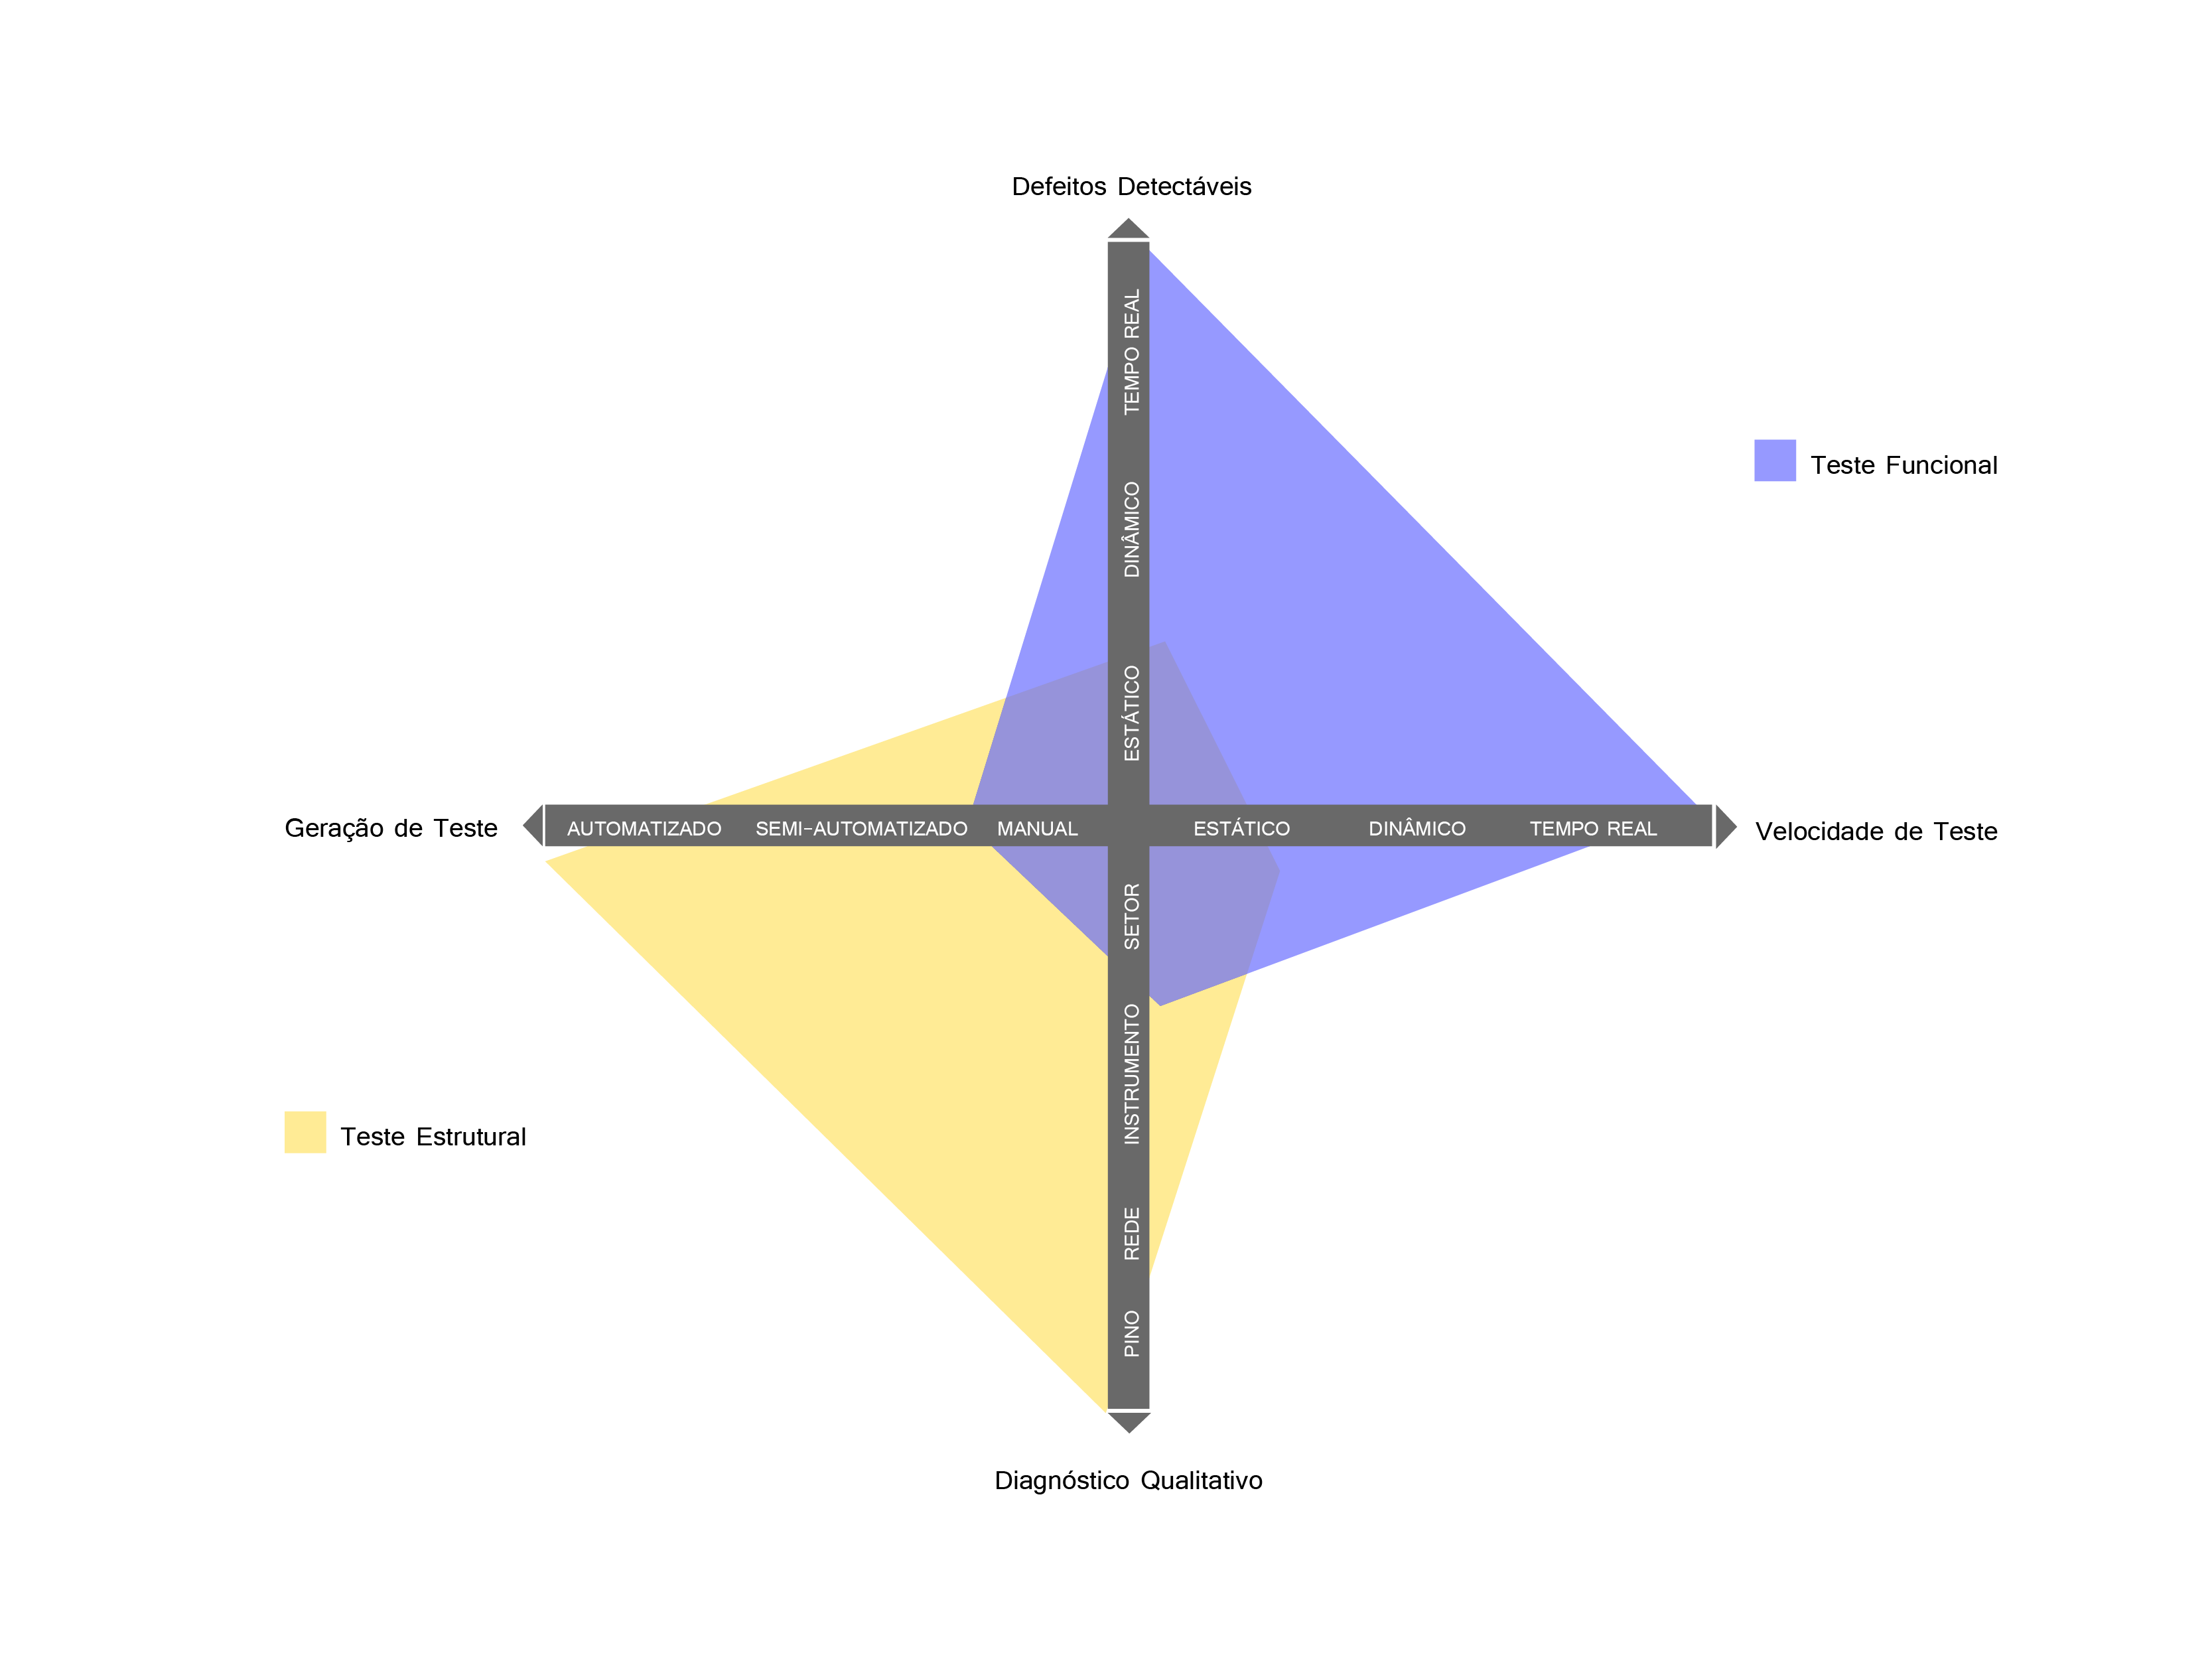
\includegraphics[width=1.2\linewidth]{coberturateste.png}
    \caption{A complementariedade dos testes estruturais e funcionais para a cobertura de teste de um dispositivo}
    \label{fig:cobertura}
\end{figure}

Segundo Jutman (2014), a própria falta de tecnologia dos aparelhos de medição e teste, resulta na impossibilidade de realizar verificações em velocidade nominal, o que impede uma cobertura de teste plena. Por sua vez, essas falhas na cobertura de teste -- que é algo dificilmente estimável -- contribui para problemas sérios de \textit{No-Failure Found (NFF)}, que são custosos para qualquer industria. Dessa forma, a pesquisa por melhores métricas de cobertura de teste, assim como na caracterização de defeitos, tornaram-se tópicos de pesquisa muito importantes.



%@article{embeddedinstrument
%How to test high-speed memory with non-intrusive embedded instruments. ASSE